The electronics that modern computers rely on contain components that operate based on quantum mechanics; however, their computational processes are still governed by classical laws. 
For this reason, they are referred to as "classical computers."\\

Quantum computing emerged from Richard Feynman’s idea that simulating quantum systems efficiently requires quantum mechanical resources \cite{Feynman1982}. 
Classical computers struggle to model complex quantum interactions due to the exponential growth of computational requirements with system size, making exact simulations infeasible beyond small systems \cite{Brown2010}. 
Quantum computers, taking advantage of quantum mechanics phenomena like superposition and entanglement, offer a natural framework for such simulations and have been demonstrated to provide exponential speedups for certain quantum systems \cite{Georgescu_2014}.

Beyond quantum simulation, curren theoretical advancements suggest that quantum algorithms can outperform classical counterparts in solving specific problems \cite{Montanaro2016}.

\section{Introduction}
%Insert definition of qubit

The physical realization of quantum computing necessitates the development of a system capable of functioning as quantum bits (qubits). 
Qubits can be implemented through various physical mechanisms; however, their practical realization remains a significant challenge due to their susceptibility to environmental interactions, which lead to decoherence and reduce their coherence time. 
Despite the diversity of possible physical implementations, any functional quantum computing system must satisfy a set of fundamental criteria. 
These requirements, known as the DiVincenzo criteria, establish the essential conditions for the construction and operation of a viable quantum computer \cite{DiVincenzo_2000}, \cite{Manenti:2023zzn}:
\begin{enumerate}
    \item The physical system used as quantum computer must comprise a set of qubits, meaning that the quantum system must be well-characterized, and scalable such that quantum
    computing can be realized.
    \item It must be possible to initialize the qubits in a reliable state, such as the ground state.
    \item The coherence time of the qubits must be longer than the typical gate time.
    \item It must be possible to implement a universal set of quantum gates.
    \item It must be possible to measure the qubits in the computational basis.
\end{enumerate}

A possible geometric representation of qubit states is given by the Bloch sphere, which offers a visualization of two level quantum systems as vectors on a unit sphere.  
A qubit state is depicted as a vector originating from the sphere’s center, with the computational basis states $\ket{0}$ and $\ket{1}$ positioned at the north and south poles, respectively.
The axis connecting these states defines the $z$-axis. The transverse $x$- and $y$- axes correspond to the equal superposition states $\ket{\pm} = \frac{1}{\sqrt{2}}(\ket{0}\pm\ket{1})$ and $\ket{\pm i} = \frac{1}{\sqrt{2}}(\ket{0}\pm i\ket{1})$, respectively.\\
A vector of unit length on the Blooch sphere is characterized by the polar angle $\theta$, with $0\leq\theta\leq\pi$ and the azimuthal angle $\varphi$, with $0\leq\varphi\leq 2\pi$, each unit vector represent a possible pure state of the qubit.\\
It can be shown that the hamiltonian of a qubit can be written as \begin{equation}\label{eq:qubithamiltonian}
    \hat{H_Q}=\hbar\omega\hat{\sigma}_z,
\end{equation} 
with $\hbar=h/2\pi$, where $h$ is the Planck's constant, $\omega$ is the qubit frequency and $\hat{\sigma}_z$ is the Pauli matrix. 

\begin{figure}[h!]
\centering
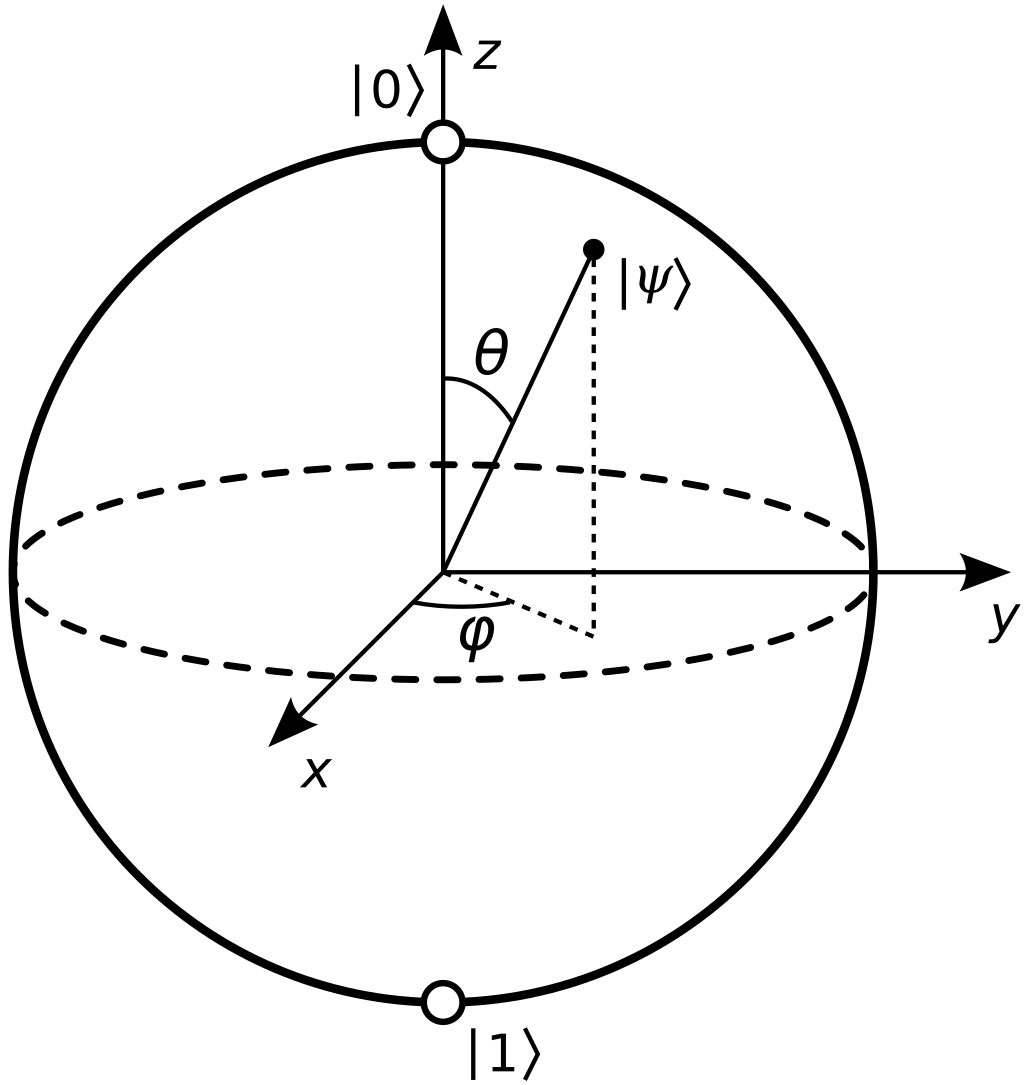
\includegraphics[width=0.25\textwidth]{figures/png/Bloch_sphere.svg.png}
\caption{Example of qubit state representation on the Bloch sphere}
\label{fig:BlochSphere}
\end{figure}

In the present work, I will focus on superconducting qubits, which constitute the hardware I have worked on and where the experiments were conducted. 
However, several of the experiments described later can also be implemented using different physical systems.

\section{Operation on qubits}

\subsection{Density matrix}
%Posso rappresentatre l'operatore densità come una matrce 2x2, mi serve per dopo, per la descrizione del depolarizing channel
\section{Quantum operations}
A quantum operation is a mathematical transformation that describes how a quantum state changes as a consequence of a physical process. Formally, it is a map $\mathcal{E}$ that transforms a quantum state described by a density operator $\hat{\rho}$ into another state described by a new density operator $\hat{\rho}'$:
\begin{equation}
    \mathcal{E}(\rho) = \rho'\label{eq:quantum_map}.
\end{equation}

The simplest example of a quantum operation is the evolution of a quantum state $\hat{\rho}$ of a closed quantum system, under a unitary operator $\hat{U}$, which can be written as $\mathcal{E} \equiv \hat{U} \hat{\rho} \hat{U}^{\dagger}$.

\paragraph{Depolarizing chennel}
A depolarizing channel describes a process in which the current state of the $n$-qubit system $\rho$, is replaced by $\frac{\id}{2^n}$, with probability $d$. This process can be represented with a quantum map as follows:
\begin{equation}
    \mathcal{E}_{dc}(\rho) = d\frac{\id}{2^n}+(1-d)\rho\label{eq:depolarizing_channel}
\end{equation} 

\section{Transmon qubit}

\subsection{Rabi experiments}

\subsection{cQED systems} \label{sec:cQED}

The frequency $f_Q$ of a two-junction transmon dependends on the magnetic flux $\Phi_Q(t)$ through the SQUID loop, for symmetric junctions is given by\cite{TransmonPaper}
\begin{equation}\label{eq:freqdepndenceonflux}
    f_Q(\Phi_Q) \approx \frac{1}{h} \left( \sqrt{8E_J E_C \cos\left(\pi \frac{\Phi_Q}{\Phi_0} \right)} - E_C \right)    
\end{equation}

where $E_C$ is the charging energy, $E_J$ is the sum of the Josephson energies of the individual Josephson junctions, $\Phi_0$ is the flux quantum, and $h$ is the Planck's constant.